% !TEX options=--shell-escape
\documentclass[10pt]{beamer}

\pdfmapfile{+sansmathaccent.map}
\newtheorem{thm}{Theorem}
\usetheme[progressbar=frametitle]{metropolis}
\usepackage{appendixnumberbeamer}

\usepackage{booktabs}
\usepackage[scale=2]{ccicons}
\usepackage{minted}

\usepackage{pgfplots}
\usepgfplotslibrary{dateplot}

\usepackage{xspace}
\newcommand{\themename}{\textbf{\textsc{metropolis}}\xspace}

\title{CS3243 - Introduction to Artificial Intelligence}
\subtitle{Tutorial 3}
% \date{\today}
\date{}
\author{Theodore Leebrant}
\institute{Tutorial Group 3}
% \titlegraphic{\hfill%\includegraphics[height=1.5cm]{logo.pdf}}

\begin{document}

\maketitle

\section[Key Concepts]{Key Concepts}

\begin{frame}[fragile]{Overview}
\begin{itemize}
  \item \textbf{Modelling a search problem}
  \begin{itemize}
    \item Define state, start/goal states, set of actions, transition model
    \item Compute size of state space
  \end{itemize}
  \item \textbf{Uninformed search space}
  \begin{itemize}
    \item Tracing
    \item Completeness
    \item Optimality
    \item Space and Time Complexity
  \end{itemize}
\end{itemize}
\end{frame}

\begin{frame}[fragile]{Modelling a Search Problem}
\begin{itemize}
  \item \textbf{State}: include essential variables ( + Initial / Goal state(s))
  \item \textbf{Actions}: possible actions that the agent can do
  \item \textbf{Transition model}: description of what each action does \\
  (specified by a function that returns a state). \\
  \verb|RESULT(STATE, ACTION) => RESULT_STATE|
  \item \textbf{Goal test}: determine whether the state is a goal state
  \item \textbf{Cost function}: a function that assigns a cost to each action
\end{itemize}
\end{frame}

\begin{frame}[fragile]{Specifying Search Space}
The search space is implicitly represented by a graph, with nodes and edges.
\begin{itemize}
  \item \textbf{Branching factor (b)}: how many actions are available at each state.
  \item \textbf{Depth}: Depth of shallowest goal node \textbf{(d)}, maximum depth of any path in the state space \textbf{(m)}.
\end{itemize}
\begin{center}
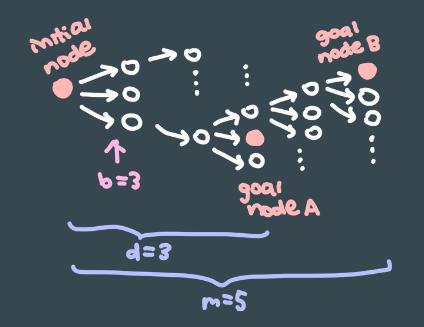
\includegraphics[width = 0.5\textwidth]{img/m_d.png}
\end{center}
\end{frame}

\begin{frame}[fragile]{Properties of cost}
The confusing lecture part - path cost

Usually, $g(n)$ is the current path cost from the initial state to node n (as defined in AIMA)

In lecture, Prof defined: \\
$g(n)$ as the \textit{optimal} path cost from initial state to n\\
$\hat{g}(n)$ as the current (minimum) path cost to n \\
$\hat{g}_{pop}(n)$ as the minimum path to n when we pop\\

Step cost - $c(s, a, s')$: the cost from $s$ to $s'$ when taking action $a$.
\end{frame}

\begin{frame}[fragile]{Uninformed Search Algorithms}
All the algorithms you learn are in the family of whatever-first search:

\begin{verbatim}
put s into data_structure
while data_structure is not empty:
    take node from data_structure
    for each neighbour:
        if goal_test:
            return true
        else:
            put neighbour into data_structure
return false
\end{verbatim}

This is a tree-based implementation without memory of searched space.
For DFS the data structure is a stack; BFS: queue; UCS: Priority queue

\end{frame}


\begin{frame}[fragile]{Uninformed Search Algorithms}
\begin{verbatim}
put s into data_structure
while data_structure is not empty:
    take node from data_structure
    mark node
    for each neighbour:
        if goal_test:
            return true
        else if neighbour unmarked:
            put neighbour into data_structure
return false
\end{verbatim}

This is the graph-based implementation.

The term whatever-first search is taken from \href{algorithms.wtf}{\underline{Jeff Erickson's Algorithm}} (and is not a term you should use in exam)
\end{frame}


\begin{frame}[fragile]{Uninformed Search Algorithms}
\textbf{BFS:} Expands shallowest node first. Use when you know \underline{solution is near root} or \underline{ree is deep but solutions are rare}. \bigskip \\ 
\textbf{UCS:} Expand the least-path-cost unexpanded node (explore cheaper nodes by current path cost first). Equivalent to BFS if all step costs are equal. It is a special case of Dijkstra's. \bigskip \\ 
\textbf{DFS:} Expand the deepest unexpanded node. Use when you don’t care how you reach a node, you just want to reach it, and when the solution/goal node is very deep, or when all solutions are at same depth
\end{frame}

\begin{frame}[fragile]{Completeness and Optimality}
\begin{itemize}
  \item \textbf{Complete:} if there is a path from start to the goal node, the algorithm will find it. 
  \item \textbf{Optimal:} always able to find the least cost solution. Implies completeness.
\end{itemize}
BFS: Complete if $b$ is finite, optimal if all step costs identical. \\
UCS: Complete and optimal if $b$ is finite and all step costs $\geq \varepsilon$ for some $\varepsilon > 0$.
\end{frame}




\end{document}